% Векторизация операций над матрицами малой размерности.
\subsection{Векторизация с помощью выделения однотипных \\ операций}\label{sec:text_4_small_matr}

Так как основной смысл векторной команды состоит в поэлементной обработке векторных данных с помощью одной и той же операции, то для выполнения векторизации необходимо выделить в коде однотипные операции, которые далее могут быть объединены в векторные команды.
В качестве примера программного контекста для анализа этого подхода будем рассматривать операции над матрицами малой размерности \cite{Bendersky2018VecMat2}.

\subsubsection{Операции для работы с малоразмерными матрицами}

Будем рассматривать следующие операции: умножение матрицы размера $8 \times 8$ на вектор, перемножение двух матриц размера $8 \times 8$, нахождение обратной матрицы размера $8 \times 8$.

Реализация неоптимизированной версии умножения матрицы $8 \times 8$ на вектор может выглядеть так, как это представлено на листинге~\ref{lst:text_4_small_matr_8x8_mul_vel_noopt}.

\begin{singlespace}
\begin{lstlisting}[caption={Невекторизованная версия умножения матрицы \\ размера $8 \times 8$ на вектор.},label={lst:text_4_small_matr_8x8_mul_vel_noopt}]
void matvec8_orig(float* __restrict m,
                  float* __restrict v,
                  float* __restrict r)
{
    for (int i = 0; i < V8; ++i)
    {
        float sum = 0.0;
        int ii = i * V8;

        for (int j = 0; j < V8; ++j)
        {
            sum = sum + m[ii + j] * v[j];
        }

        r[i] = sum;
     }
}
\end{lstlisting}
\end{singlespace}

Рассмотрим некоторые моменты реализации.
Матрица хранится в сплошной области памяти по строкам и передается в фунцию через указатель на начало этой области.
Все параметры функции передаются c указанием \texttt{\_\_restrict} для облегчения компилятору задачи по оптимизации.
Умножение матрицы на вектор состоит в вычислении скалярного произведения каждой строки этой матрицы на вектор и составлении из результатов выходного вектора.
Так как в рассматриваемом случае на листинге~\ref{lst:text_4_small_matr_8x8_mul_vel_noopt} размер строки матрицы равен 8 элементам типа float, то одной операцией в 512-битный регистр можно загрузить из памяти сразу 2 соседние строки матрицы.
После чего нужно выполнить операцию упакованного умножения на регистр, содержащий две копии вектора, на который умножается матрица (выполнить запись двух копий вектора в zmm регистр можно с помощью операции gather).
Сумма первых восьми элементов получившегося регистра и последних восьми элементов будут являться элементами выходного вектора $r$ (см. рис.~\ref{fig:text_4_small_matr_matvec8}).

\begin{figure}[ht]
\centering
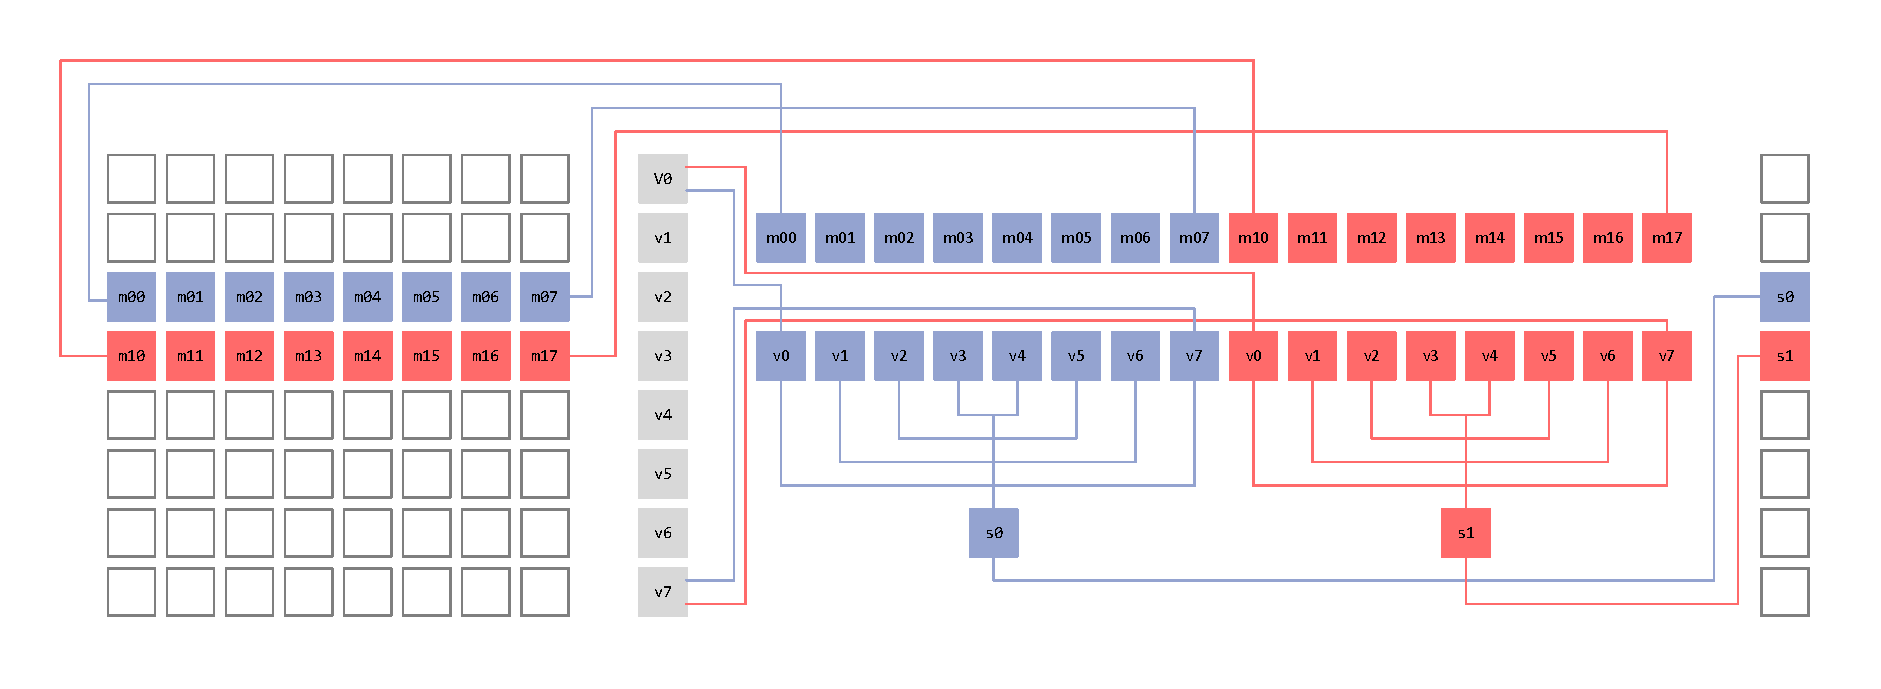
\includegraphics[width=1.0\textwidth]{./pics/text_4_small_matr/matvec8.pdf}
\singlespacing
\captionstyle{center}\caption{Схема вычисления результата в операции \texttt{matvec8}.}
\label{fig:text_4_small_matr_matvec8}
\end{figure}

Итак, при реализации операции умножения матрицы $8 \times 8$ на вектор мы должны загрузить всю матрицу в четыре zmm регистра.
Затем выполнить четыре упакованные операции умножения этих регистров, на регистр, содержащий две копии вектора, на которые умножается матрица.
После этого из каждого из получившихся четырех регистров мы должны получить сумму элементов каждой его половины, что в результате даст 8 искомых элементов выходного вектора.
Получение суммы элементов половины zmm регистра представляет собой горизонтальную операцию, реализация которой с помощью интринсика оказывается слишком дорогой.
Как показали эксперименты, простое применение интринсика \texttt{\_mm512\_mask\_reduce\_add\_ps} (и даже безмасочного \texttt{\_mm512\_reduce\_add\_ps} в случае умножения матрицы $16 \times 16$) не приводит к ускорению по сравнению с оригинальной версией функции, оптимизированной компилятором icc с использованием уровня оптимизации -O3.
Прежде чем переходить к оптимизации горизонтальных операций сложения рассмотрим второй интересующий нас пример, -- перемножение двух матриц размера $8 \times 8$, -- с целью выделения похожих однотипных операций.

Как и в случае с примером умножения матрицы на вектор, вначале приведем простую реализацию неоптимизированной версии перемножения двух матриц размера $8 \times 8$ (листинг~\ref{lst:text_4_small_matr_8x8_mul_matr_noopt}):

\begin{singlespace}
\begin{lstlisting}[caption={Невекторизованная версия перемножения матриц \\ размера $8 \times 8$.}, label={lst:text_4_small_matr_8x8_mul_matr_noopt}]
void matmat8_orig(float* __restrict a,
                  float* __restrict b,
                  float* __restrict r)
{
    for (int i = 0; i < V8; ++i)
    {
        int ii = i * V8;
 
        for (int j = 0; j < V8; ++j)
        {
            float sum = 0.0;

            for (int k = 0; k < V8; ++k)
            {
                int kk = k * V8;
                
                sum = sum + a[ii + k] * b[kk + j];
            }

            r[ii + j] = sum;
        }
    }
}
\end{lstlisting}
\end{singlespace}

Логика перемножения двух матриц состоит в том, что результаты попарного скалярного произведения 8 строк матрицы $a$ и 8 столбцов матрицы $b$ формируют элементы результирующей матрицы.
Как и в случае умножения матрицы на вектор, использование 512-битных команд загрузки данных из памяти позволяет за одну операцию загрузить две соседние строки матрицы $a$ (операцией последовательного чтения) или два соседних столбца матрицы $b$ (с помощью операции gather).
После этого мы должны вычислить четыре скалярные произведения каждой половины загруженного из матрицы $a$ вектора с каждой половиной загруженного из матрицы $b$ вектора.
Для этого выполняются две операции поэлементного перемножения двух загруженных векторов, в одном из которых старшая и младшая половины второго вектора переставлены местами, как показано на рис.~\ref{fig:text_4_small_matr_matmat8}.

\begin{figure}[ht]
\centering
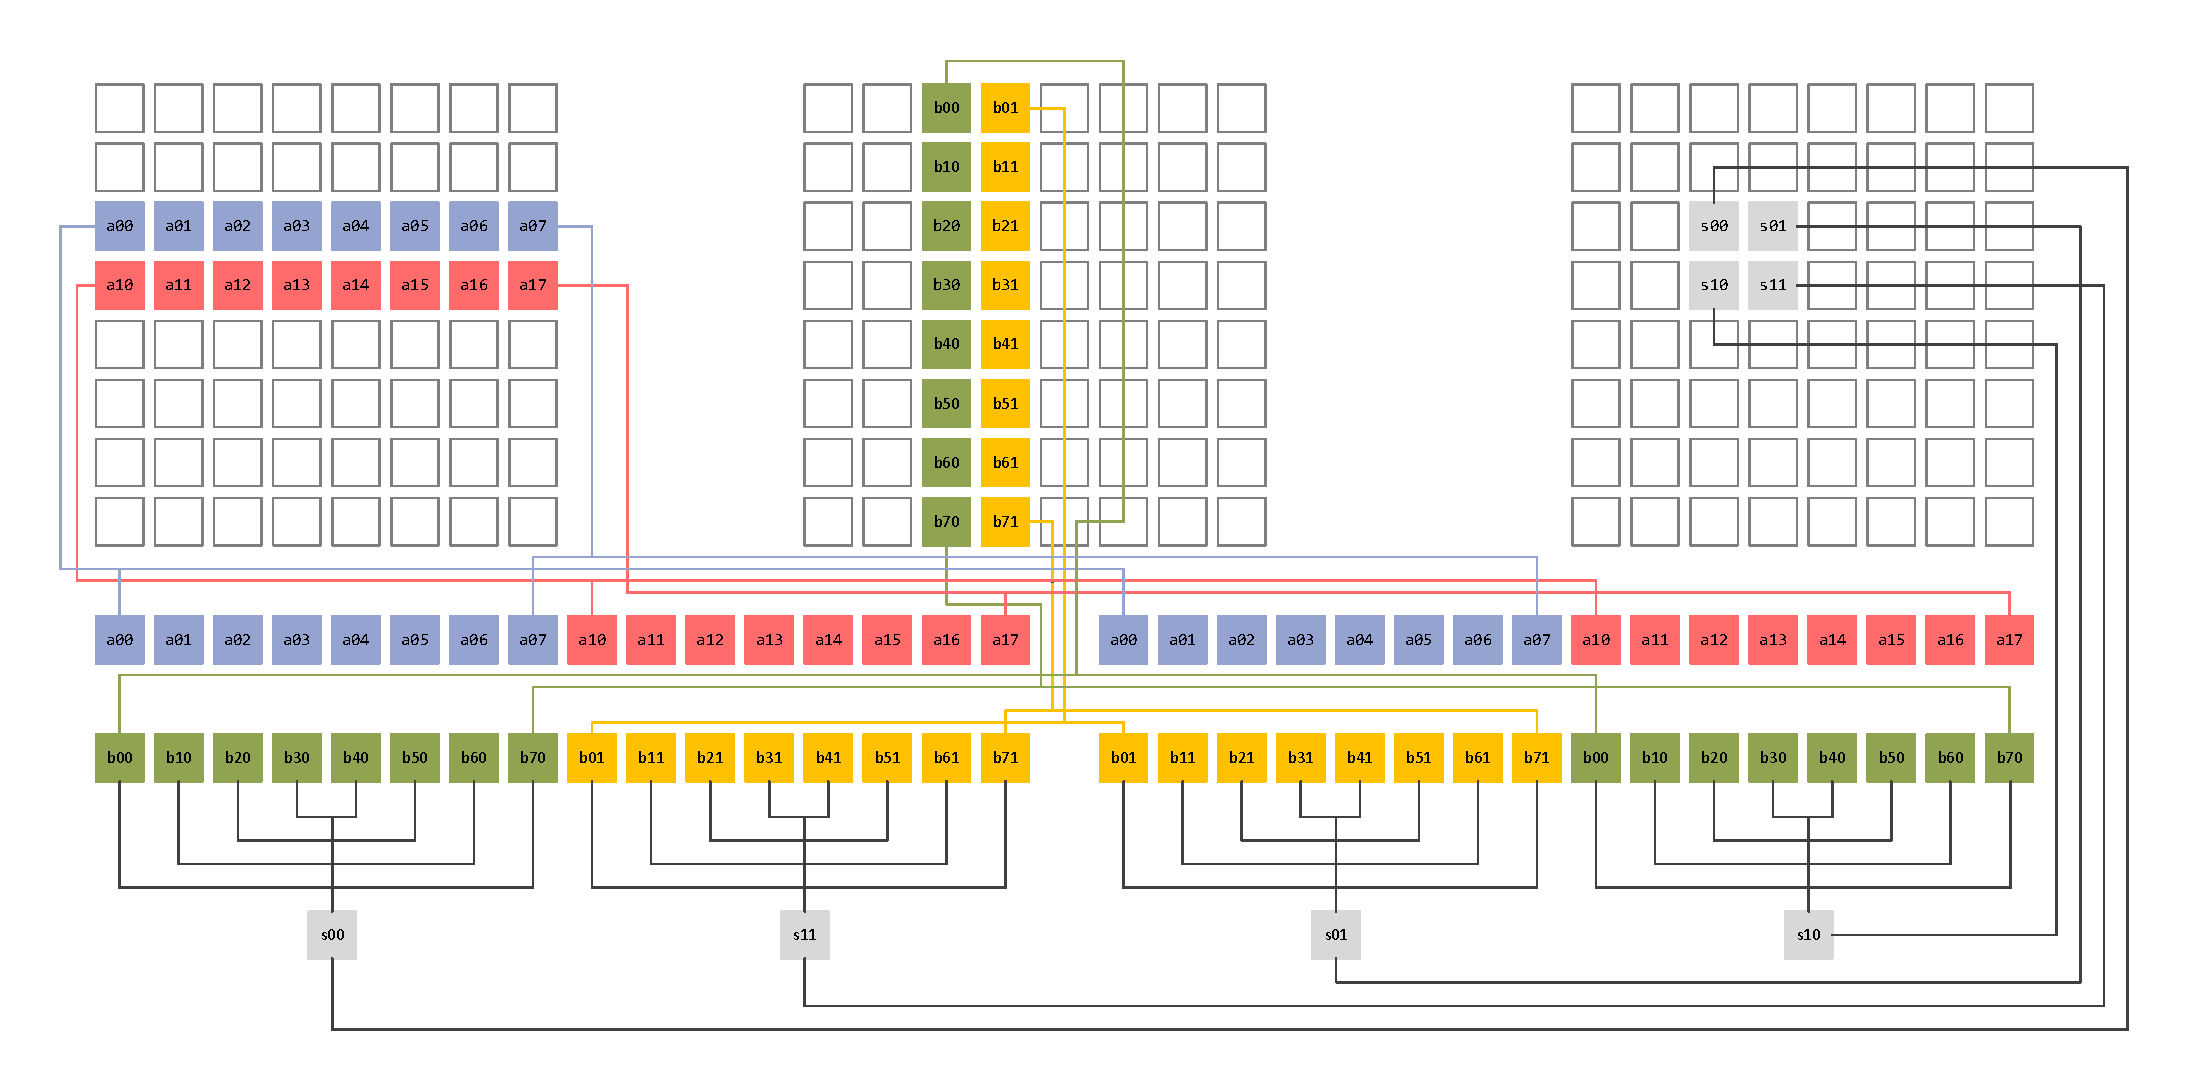
\includegraphics[width=1.00\textwidth]{./pics/text_4_small_matr/matmat8.pdf}
\singlespacing
\captionstyle{center}\caption{Схема вычисления результата в операции \texttt{matmat8}.}
\label{fig:text_4_small_matr_matmat8}
\end{figure}

После выполнения действий, представленных на рис.~\ref{fig:text_4_small_matr_matmat8}, возникает потребность вычисления суммы 8 младших элементов вектора и 8 старших элементов этого же вектора.
Таким образом, мы приходим к тому, что каждый элемент результирующей матрицы должен быть получен с помощью горизонтальной операции суммирования 8 младших или старших элементов некоторого zmm регистра.

Примеры реализаций функций \texttt{matvec16\_orig} и \texttt{matmat16\_orig} аналогичны, но там возникают задачи суммирования всех 16 элементов вектора.
Отсюда возникает потребность объединения таких горизонтальных операций вместе.
Рассмотрим задачу в общем виде: даны 16 zmm регистров (a, b, c, d, e, f, g, h, i, j, k, l, m, n, o, p), каждый из которых содержит по 16 элементов типа float.
Требуется посчитать суммы их элементов и записать в один регистр zmm.
Набор команд AVX-512 и библиотека интринсиков содержат все необходимые возможности для эффективной реализации этого функционала.
Схема вычислений состоит из четырех фаз, каждая из которых реализуется операциями перестановок с последующим сложением и слиянием векторов.

\begin{figure}[!ht]
\centering
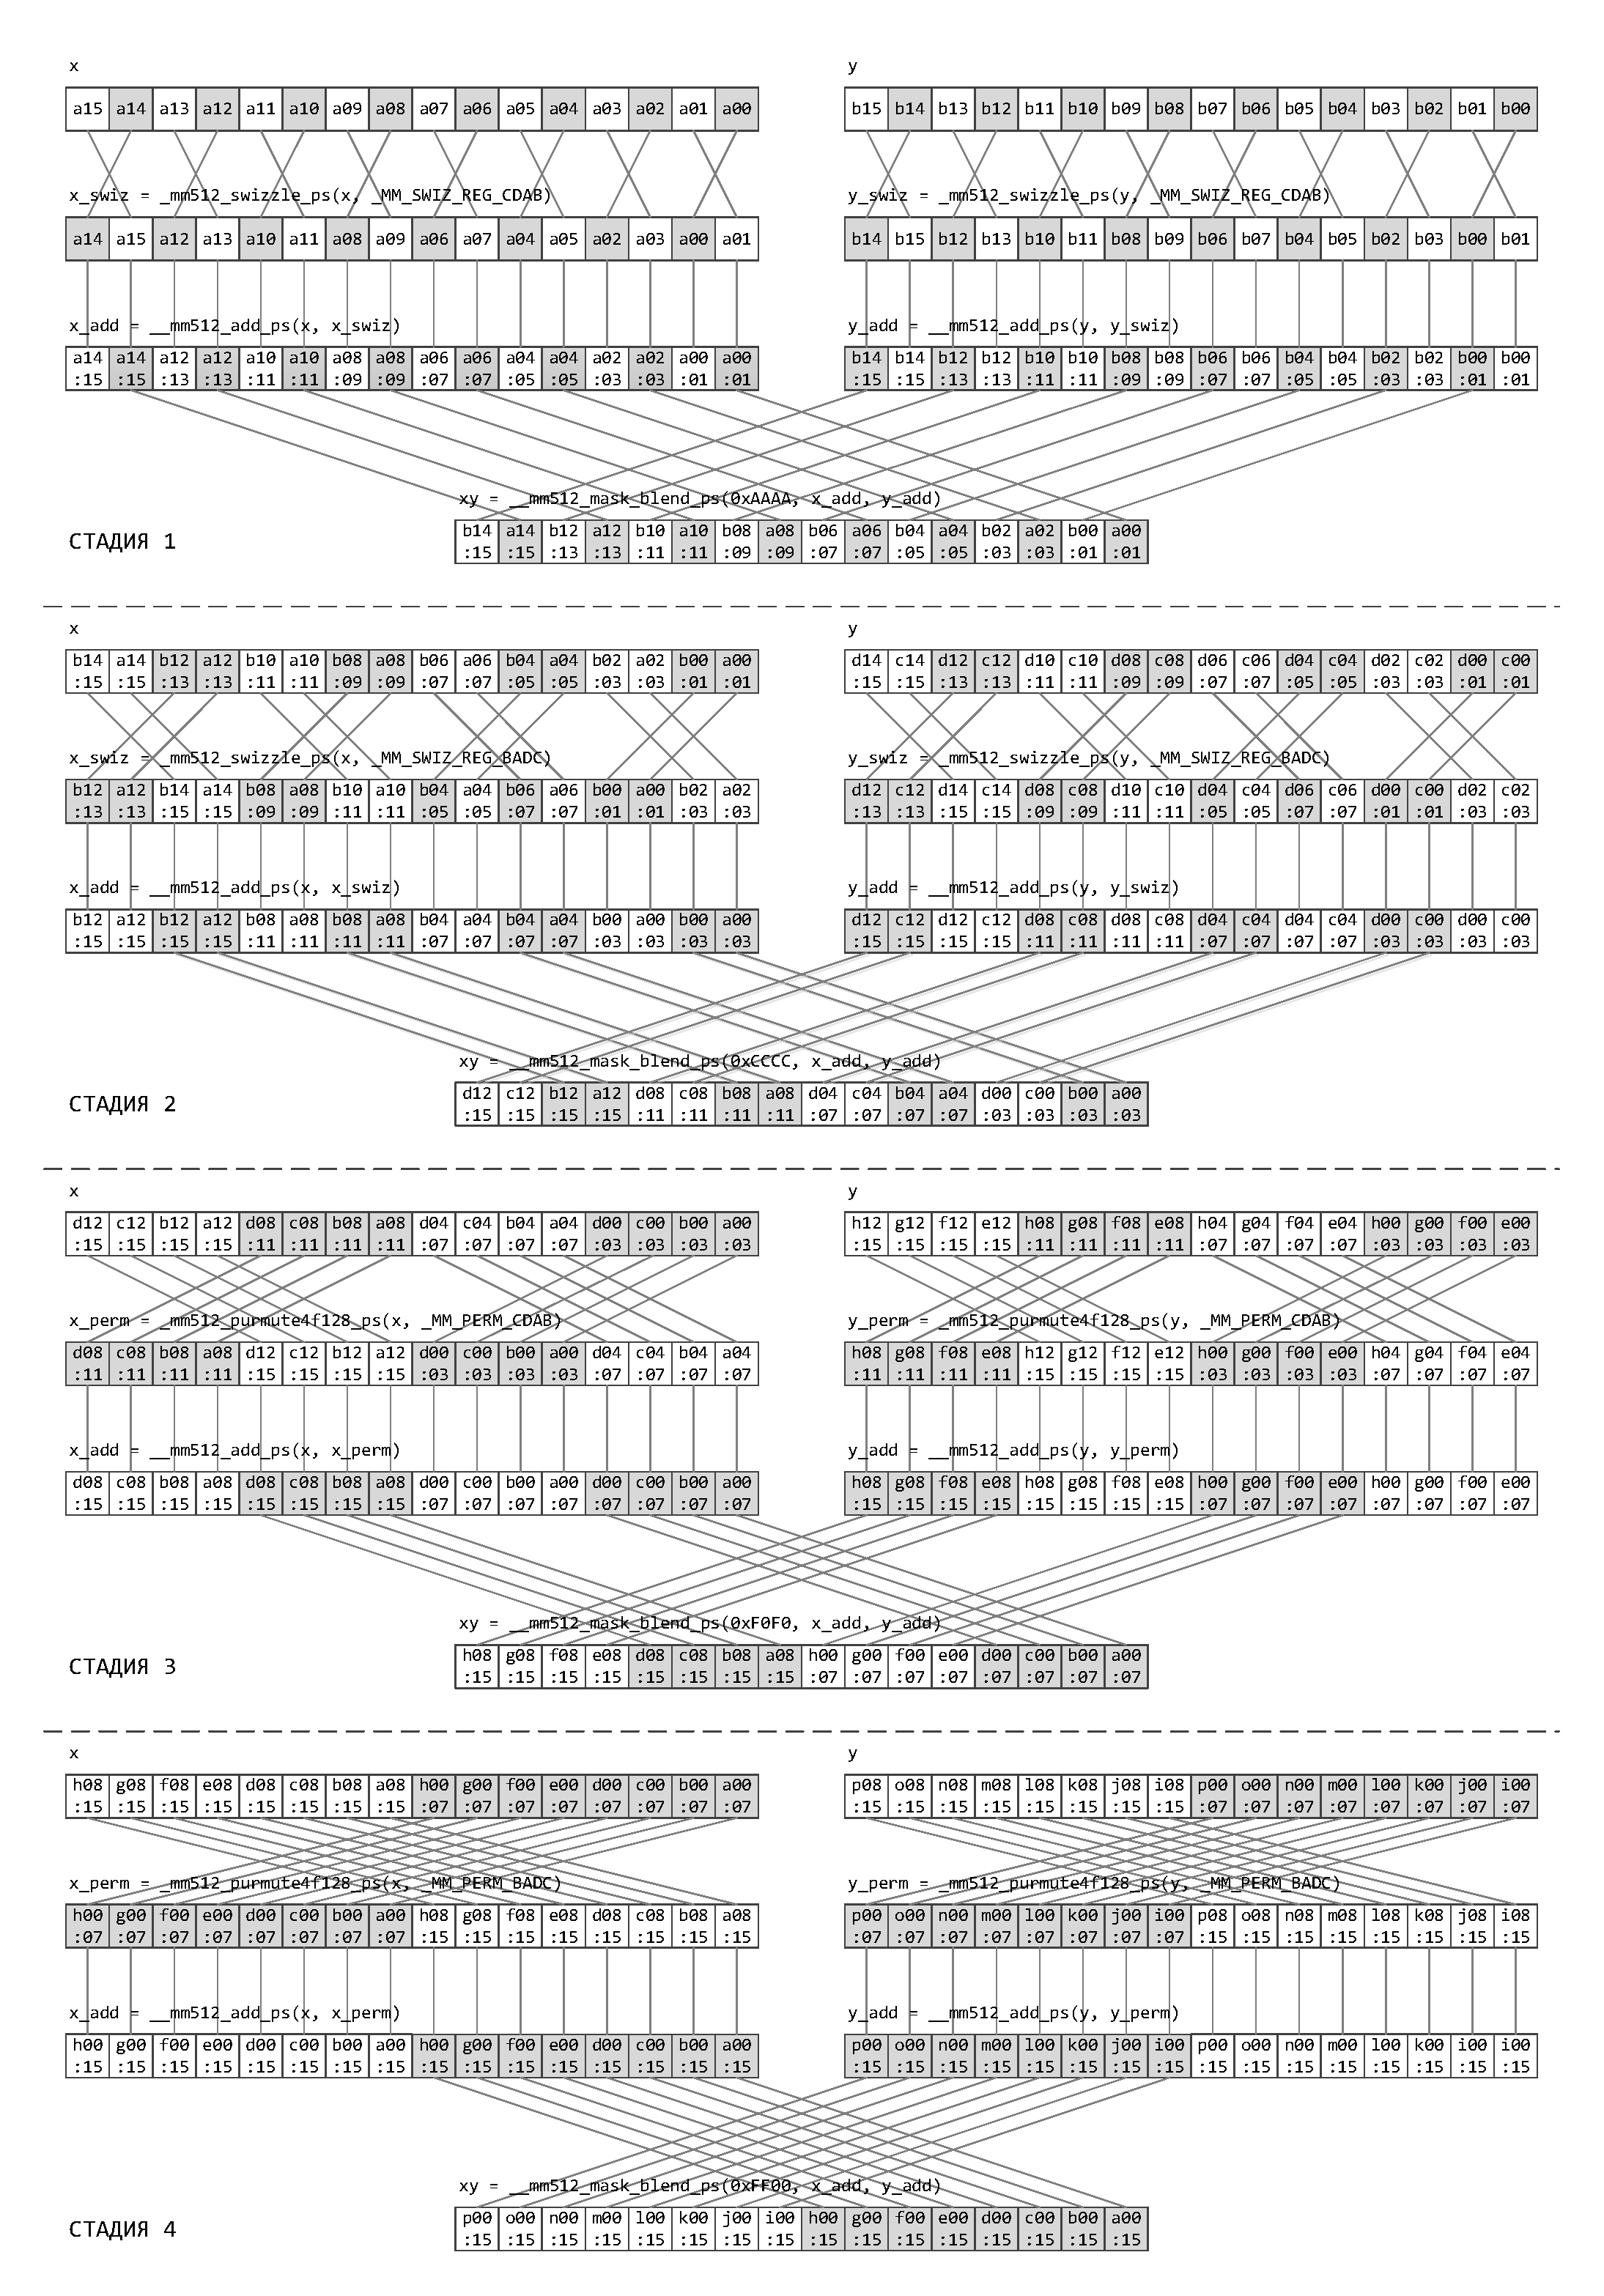
\includegraphics[width=0.95\textwidth]{./pics/text_4_small_matr/horizontal_add.pdf}
\singlespacing
\captionstyle{center}\caption{Схема суммирования элементов zmm вектора.}
\label{fig:text_4_small_matr_horizontal_add}
\end{figure}

На рис.~\ref{fig:text_4_small_matr_horizontal_add} представлена схема суммирования элементов для пары векторов (a и b).

Набор команд AVX-512 не содержит операций горизонтального сложения элементов вектора zmm.
Таким образом, для сложения двух элементов одного и того же вектора требуется покомпонентно сложить этот вектор со своей копией, в которой элементы переставлены нужным образом.
Это действие и выполняется на каждой обозначенной на рис.~\ref{fig:text_4_small_matr_horizontal_add} фазе.
Так как всего вектор содержит 16 элементов, то минимальное количество фаз, необходымых для суммирования его элементов равно 4.
После первой фазы (после выполнения операции слияния blend) можно наблюдать вектор, содержащий суммы пар соседних элементов векторов a и b, после второй фазы вектор состоит уже из сумм четверок элементов векторов a, b, c и d, и т. д.

\begin{figure}[ht]
\centering
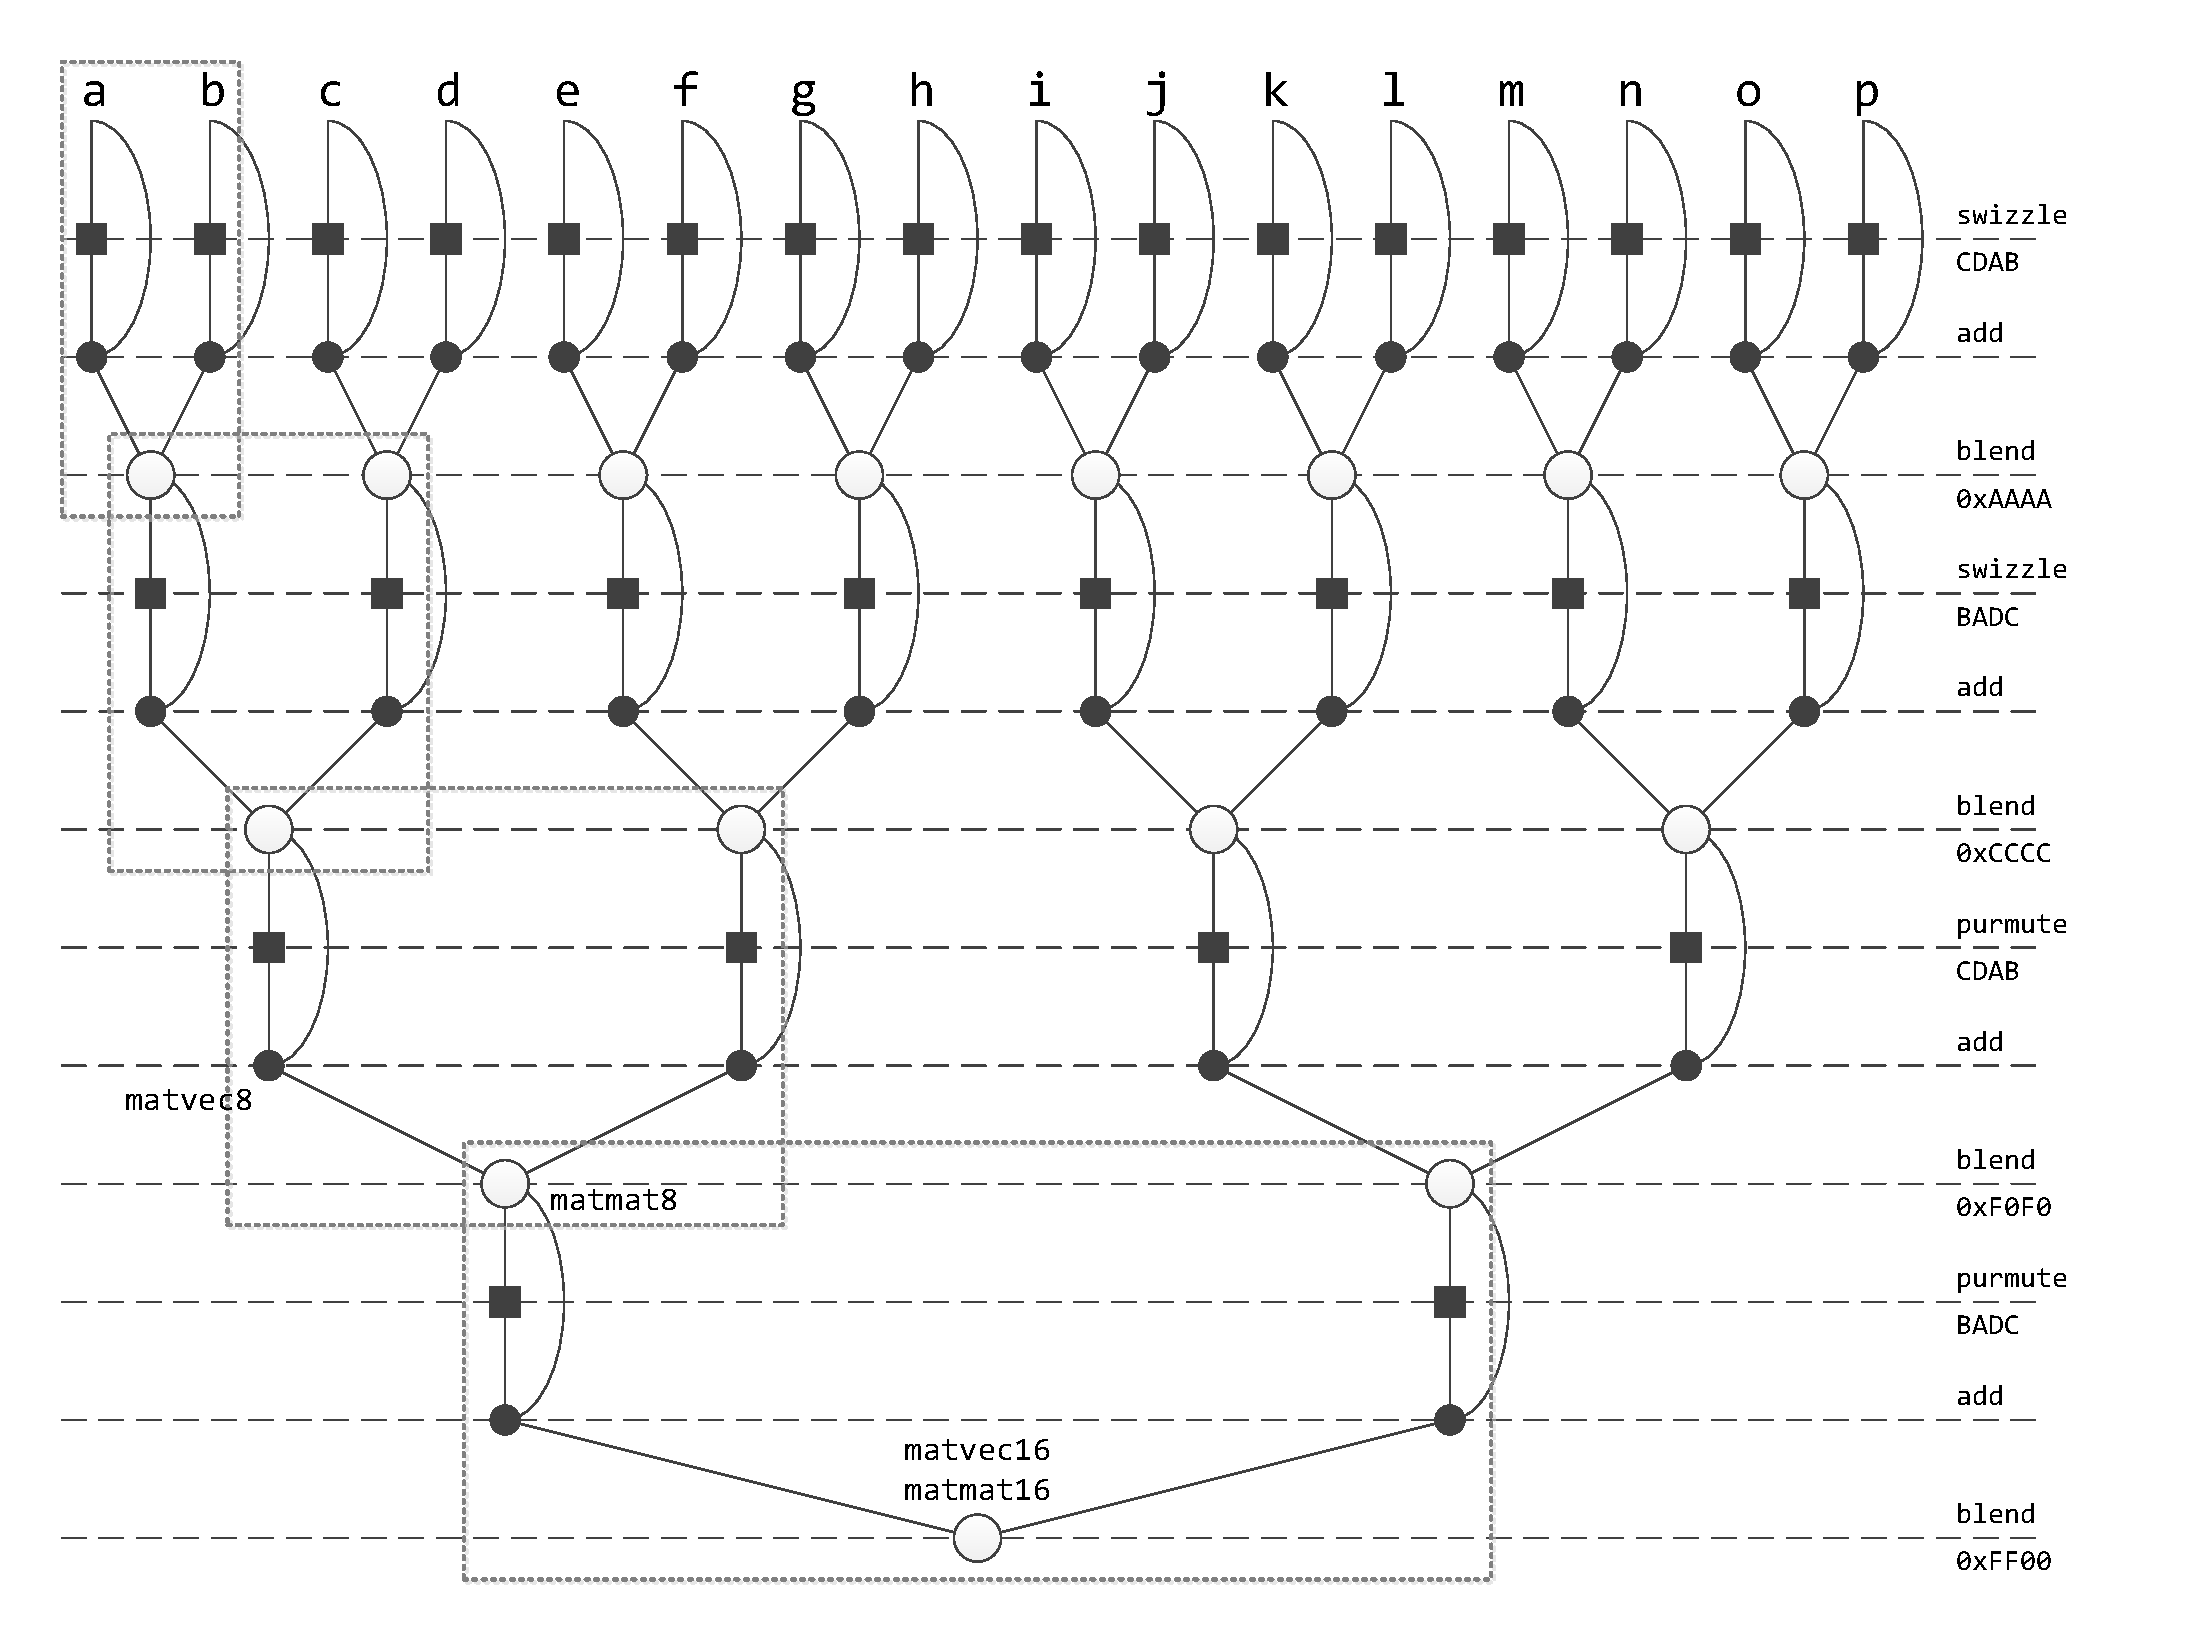
\includegraphics[width=0.8\textwidth]{./pics/text_4_small_matr/operations_tree.pdf}
\singlespacing
\captionstyle{center}\caption{Схема суммирования элементов 16 zmm векторов.}
\label{fig:text_4_small_matr_operations_tree}
\end{figure}

На рис~\ref{fig:text_4_small_matr_operations_tree} представлен граф потока данных для осуществления суммирования всех элементов 16 векторов.
При этом черными квадратами обозначены операции перестановки элементов (swizzle или permute в терминах интринсиков), черными кругами обозначены операции сложения вектора со своей пермутированной копией, а белые круги обозначают операции слияния двух векторов по маске.
Прямоугольниками с пунктирной границей очерчены стадии из рис.~\ref{fig:text_4_small_matr_horizontal_add}.

Можно заметить, что граф потока данных на рис.~\ref{fig:text_4_small_matr_operations_tree} состоит из схожих блоков операций, выполняющих одни и те же действия с разными входными регистрами: пермутация двух векторов, сложение пары векторов с пермутированной копией и слияние этих двух результатов по маске (2 swizzle/permute + 2 add + 1 blend).
Причем на каждой фазе свои маски перестановок и слияний, но они постоянны для всех входных векторов.
Для удобства можно определить макросы, реализующие обозначенные фазы.
На вход макрос получает пару обрабатываемых векторов, а также параметры перестановки элементов и слияния результирующей пары.
Пара макросов объясняется тем, что интринсик swizzle предназначен для перестановки элементов внутри 128-битных четвертей, а permute4f128 переставляет местами эти четверти (обе функции раскрываются в операцию perm).

\begin{singlespace}
\begin{lstlisting}[caption={Определение макросов для реализации фаз суммирования элементов векторов.}, label={lst:text_4_small_matr_swiz_macro}]
#define SWIZ_2_ADD_2_BLEND_1(X, Y, SWIZ_TYPE, BLEND_MASK)\
    _mm512_mask_blend_ps(BLEND_MASK,\
        _mm512_add_ps(X, _mm512_swizzle_ps(X, SWIZ_TYPE)),\
        _mm512_add_ps(Y, _mm512_swizzle_ps(Y, SWIZ_TYPE)))

#define PERM_2_ADD_2_BLEND_1(X, Y, PERM_TYPE, BLEND_MASK)\
    _mm512_mask_blend_ps(BLEND_MASK,\
        _mm512_add_ps(X, _mm512_permute4f128_ps(X, PERM_TYPE)),\
        _mm512_add_ps(Y, _mm512_permute4f128_ps(Y, PERM_TYPE)))
\end{lstlisting}
\end{singlespace}

Есть еще один похожий вариант выполнения одной фазы, реализующийся последовательностью операций 2 swizzle/permute + 2 blend + 1 add, но он оказался менее эффективным, поэтому не приводится.

Последний рассматриваемый в разделе пример -- нахождение обратной матрицы.
Приведем краткое описание алгоритма Гаусса-Жордана для нахождения обратной матрицы\label{term:alg_gauss_zhordan} и опишем пути оптимизации реализации соответствующей функции \texttt{invmat8\_orig}.

По алгоритму Гаусса-Жордана к исходной матрице $m$ нужно приписать справа единичную матрицу $e$.
Получим прямоугольную матрицу вида ($m|e$), размера $8 \times 16$.
Далее над этой матрицей необходимо выполнить такие преобразования строк (перестановка строк, умножение строки на число, прибавление к одной строке другой строки, умноженной число), чтобы исходная матрица, стоящая слева, трансформировалась в единичную.
Тогда матрица, стоящая справа, из единичной трансформируется в искомую обратную матрицу.
Для достижения этого эффекта выполняется следующая последовательность действий (цикл по $i$ от 0 до 8):

\begin{figure}[ht]
\centering
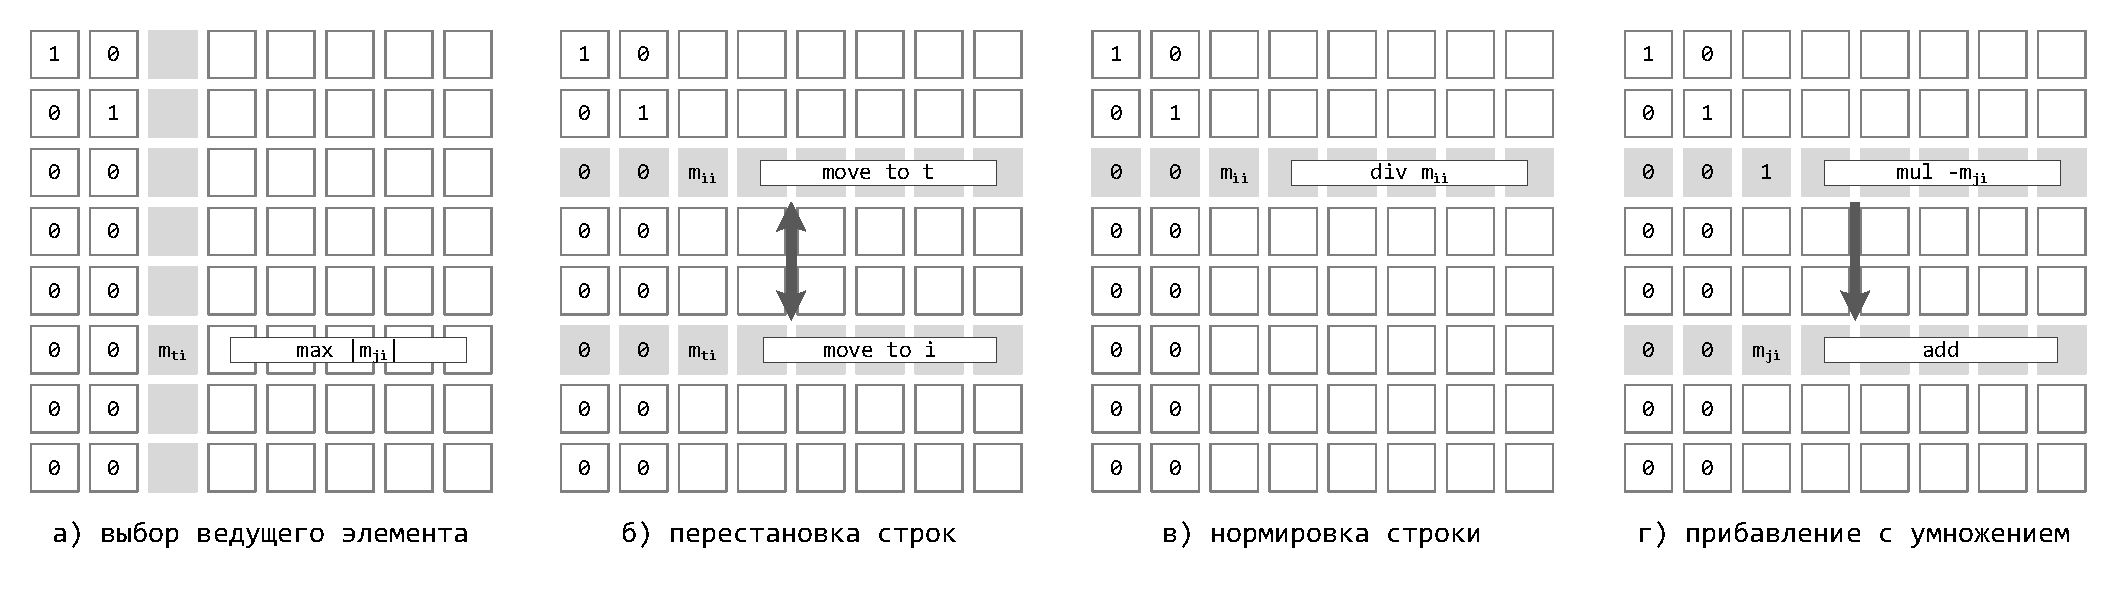
\includegraphics[width=1.0\textwidth]{./pics/text_4_small_matr/invmat8.pdf}
\singlespacing
\captionstyle{center}\caption{Базовые действия алгоритма Гаусса-Жордана нахождения обратной матрицы.}
\label{fig:text_4_small_matr_invmat8}
\end{figure}

Поиск ведущей строки с максимальным абсолютным значением $i$-го элемента (рис.~\ref{fig:text_4_small_matr_invmat8}, а).
Если такое значение равно нулю, то матрица вырождена.
Это единственное место алгоритма, которое плохо поддается векторизации, к тому же содержит аварийный выход.

Перестановка ведущей строки и $i$-ой строки местами (рис.~\ref{fig:text_4_small_matr_invmat8}, б).
После выполнения этого действия элемент $m_{ii}$ является максимальным по абсолютному значению элементом $i$-го столбца.
Действие успешно векторизуется с помощью операций пересылки zmm векторов.

Нормировка $i$-ой строки матрицы, то есть деление всех ее элементов на $m_{ii}$ (рис.~\ref{fig:text_4_small_matr_invmat8}, в).
После выполнения этого действия элемент $m_{ii}$ равен единице.
Реализуется одной операцией упакованного деления (или упакованного умножения на обратный элемент).

С помощью $i$-ой строки обнуление всех $i$-ых элементов во всех остальных строках (рис.~\ref{fig:text_4_small_matr_invmat8}, г).
Выполняется путем прибавления $i$-ой строки, умноженной на нужный коэффициент, к каждой строке матрицы.
Для этого действия применяются упакованные FMA\label{abbr:fma} операции, которые существенно ускоряют код.

Однако нужно сделать одну оговорку.
Описанные выше действия выполняются над строками матрицы размера $8 \times 16$, последовательно хранящейся в памяти.
Но на вход функции подается матрица $8 \times 8$, также хранящаяся в памяти последовательно.
Поэтому внутри функции возникают накладные действия, связанные с копированием элементов входной матрицы во временную матрицу $8 \times 16$ и обратным копированием из временной матрицы результата.
Также требуется инициализация правой части временной матрицы элементами единичной матрицы.
Все эти накладные действия реализуются с помощью операций gather/scatter.
Заметим, что при реализации \texttt{invmat16} накладные расходы не обязательны, так как нет смысла объединять две матрицы $16 \times 16$ в одну временную матрицу $16 \times 32$ (строка объединенной матрицы, содержащая 32 значения типа float, все равно не поместится в zmm регистр).

\subsubsection{Векторная реализация операций над малоразмерными \\ матрицами}\label{sec:text_4_small_matr_realization}

Приведем оптимизированные фрагменты для описанных операций с матрицами размера $8 \times 8$.
В реализации функции \texttt{matvec8\_opt} следует отметить загрузку двух копий вектора в zmm регистр с помощью операции gather.
Существует возможность загрузки двух копий 256-битного участка памяти в zmm регистр, однако реализована она с помощью функции-интринсика \texttt{\_mm512\_extload\_pd} с указанием параметра \texttt{\_MM\_BROADCAST\_4X8}.
Так как формально в данном случае результатом является регистр типа \texttt{\_\_m512d}, то было решено оставить чтение через gather.
Выполнение горизонтальных операций суммирования половинок четырех zmm регистров заканчивается на операции add третьей фазы, как показано на рис.~\ref{fig:text_4_small_matr_horizontal_add} (см. листинг~\ref{lst:text4_small_matr_matvec_opt}).

\begin{singlespace}
\begin{lstlisting}[caption={Векторизованная версия умножения матрицы \\ размера $8 \times 8$ на вектор.}, label={lst:text4_small_matr_matvec_opt}]
void matvec8_opt(float* __restrict m,
                 float* __restrict v,
                 float* __restrict r)
{
  ...
  ind_gth = _mm512_set_epi32(7,6,5,4,3,2,1,0,7,6,5,4,3,2,1,0);
  ind_sct = _mm512_set_epi32(0,0,0,0,7,5,3,1,0,0,0,0,6,4,2,0);
  ...
  vec = _mm512_i32gather_ps(ind_gth, v, _MM_SCALE_4);
  ...
  m0 = _mm512_mul_ps(_mm512_load_ps(&m[0]), vec);
  ...
  x0 = SWIZ_2_ADD_2_BLEND_1(m0, m2, _MM_SWIZ_REG_CDAB, 0xAAAA);
  x2 = SWIZ_2_ADD_2_BLEND_1(m4, m6, _MM_SWIZ_REG_CDAB, 0xAAAA);
  m0 = SWIZ_2_ADD_2_BLEND_1(x0, x2, _MM_SWIZ_REG_BADC, 0xCCCC);
  x0 = _mm512_add_ps(m0, _mm512_permute4f128_ps(m0, _MM_PERM_CDAB));
  ...
  _mm512_mask_i32scatter_ps(r, 0xF0F, ind_sct, x0, _MM_SCALE_4);
}
\end{lstlisting}
\end{singlespace}

Перемножение двух матриц изначально реализуется гнездом из трех вложенных циклов.
Два внешних цикла относятся к проходу по строкам одной из перемножаемых матриц и столбцам другой (за одну итерацию обрабатывается по две строки и по два столбца соответственно).
Во внутреннем цикле вычисляется скалярное произведение соответствующей строки и столбца.
Так как строки матрицы занимают в памяти последовательные участки, то чтение двух соседних строк выполняется обычной функцией \texttt{\_mm512\_load\_ps}.
Загрузку же двух соседних столбцов следует выполнять с использованием gather и заданными смещениями всех элементов.
По этой причине в реализации была выполнена перестановка двух внешних циклов, чтобы чтение с помощью gather выполнялось во внешнем цикле, так как эта операция более медленная, чем чтение последовательного участка памяти.
Далее выполняется полная раскрутка ставшего теперь уже внутренним цикла, проходящего по строкам матрицы $a$.
Выполнение горизонтальных операций суммирования половинок 8 регистров zmm заканчивается на операции blend третьей фазы из рис.~\ref{fig:text_4_small_matr_horizontal_add}.
Полученные 16 элементов результирующей матрицы записываются в память с использованием scatter с указанием смещений (см. листинг~\ref{lst:text_4_small_matr_matmat_opt}).

\begin{singlespace}
\begin{lstlisting}[caption={Векторизованная версия перемножения \ \\ матриц размера $8 \times 8$.}, label={lst:text_4_small_matr_matmat_opt}]
void matmat8_opt(float* __restrict a,
                 float* __restrict b,
                 float* __restrict r)
{
 ...
 ind = _mm512_set_epi32(7*V8+1, 6*V8+1, 5*V8+1, 4*V8+1,
                        3*V8+1, 2*V8+1,   V8+1,      1,
                        7*V8,   6*V8,   5*V8,   4*V8,
                        3*V8,   2*V8,     V8,        0);

 for (int j = 0; j < V8; j += 2)
 {
  ...
  bj = _mm512_i32gather_ps(ind, &b[j], _MM_SCALE_4);
  bj2 = _mm512_permute4f128_ps(bj, _MM_PERM_BADC);
  ...
  a0 = _mm512_load_ps(&a[ii0]);
  m0 = _mm512_mul_ps(a0, bj);
  m1 = _mm512_mul_ps(a0, bj2);
  ...
  x0 = SWIZ_2_ADD_2_BLEND_1(m0, m1, _MM_SWIZ_REG_CDAB, 0xAAAA);
  x1 = SWIZ_2_ADD_2_BLEND_1(m2, m3, _MM_SWIZ_REG_CDAB, 0xAAAA);
  x2 = SWIZ_2_ADD_2_BLEND_1(m4, m5, _MM_SWIZ_REG_CDAB, 0xAAAA);
  x3 = SWIZ_2_ADD_2_BLEND_1(m6, m7, _MM_SWIZ_REG_CDAB, 0xAAAA);
  m0 = SWIZ_2_ADD_2_BLEND_1(x0, x1, _MM_SWIZ_REG_BADC, 0xCCCC);
  m1 = SWIZ_2_ADD_2_BLEND_1(x2, x3, _MM_SWIZ_REG_BADC, 0xCCCC);
  x0 = PERM_2_ADD_2_BLEND_1(m0, m1, _MM_PERM_CDAB, 0xF0F0);
  ...
  ind1 = _mm512_set_epi32(ii3+V8+j, ii3+V8+j+1,
                          ii2+V8+j, ii2+V8+j+1,
                          ii1+V8+j, ii1+V8+j+1,
                          ii0+V8+j, ii0+V8+j+1,
                          ii3+j+1,  ii3+j,
                          ii2+j+1,  ii2+j,
                          ii1+j+1,  ii1+j,
                          ii0+j+1,  ii0+j),
  _mm512_i32scatter_ps(r, ind1, x0, _MM_SCALE_4);
}
\end{lstlisting}
\end{singlespace}

Реализация функции \texttt{invmat8\_opt} начинается с формирования временной матрицы размера $8 \times 16$, левой частью которой становится входная матрица, а в правой считается результат (копирование входной матрицы с помощью пар операций load -- scatter и инициализация правой части).
После инициализации временной матрицы выполняется тело алгоритма Гаусса-Жордана нахождения обратной матрицы.
Действие по нахождению ведущей строки не подвергалось векторизации.
Три остальные действия реализуются без каких бы то ни было особенностей с помощью применения пересылок и покомпонентных операций сложения, умножения и комбинированных FMA операций.

\begin{singlespace}
\begin{lstlisting}[caption={Векторизованная версия вычисления обратной \\ матрицы размера $8 \times 8$.},label={lst:text_4_small_matr_invmat_opt}]
int invmat8_opt(float* __restrict m, float* __restrict r)
{
  z0 = _mm512_setzero_ps();
  z1 = _mm512_set1_ps(1.0);
  ind1 = _mm512_set_epi32(V16+7,V16+6,V16+5,V16+4,V16+3,V16+2,V16+1,V16,
                          7,6,5,4,3,2,1,0);
  ind2 = _mm512_set_epi32(0,0,0,0,0,0,0,0,
                          7*V16+7,6*V16+6,5*V16+5,4*V16+4,
                          3*V16+3,2*V16+2,V16+1,0);

  for (int i = 0; i < V8; i += 2)
  {
    _mm512_i32scatter_ps(&t[i * V16], ind1, _mm512_load_ps(&m[i * V8]),
                         _MM_SCALE_4);
    _mm512_i32scatter_ps(&t[i * V16 + V8], ind1, z0, _MM_SCALE_4);
  }

  _mm512_mask_i32scatter_ps(&t[V8], 0xFF, ind2, z1, _MM_SCALE_4);

  for (int i = 0; i < V8; ++i)
  {
    ...
    if (lead_i != i)
    {
      vi = _mm512_load_ps(&t[ii]);
      vl = _mm512_load_ps(&t[lead_i * V16]);
      _mm512_store_ps(&t[lead_i * V16], vi);
      _mm512_store_ps(&t[ii], vl);
    }
    ...
    vd = _mm512_set1_ps(1.0 / t[ii + i]);
    vi = _mm512_load_ps(&t[ii]);
    vi = _mm512_mul_ps(vi, vd);
    _mm512_store_ps(&t[ii], vi);
    ...
    for (int j = 0; j < V8; ++j)
    {
      int jj = j * V16;
      if (j != i)
      {
        vd = _mm512_set1_ps(-t[jj + i]);
        vj = _mm512_load_ps(&t[jj]);
        vi = _mm512_load_ps(&t[ii]);
        vj = _mm512_fmadd_ps(vi, vd, vj);
        _mm512_store_ps(&t[jj], vj);
      }
    }
  }

  ...
  for (int i = 0; i < V8; i += 2)
  {
    vi = _mm512_i32gather_ps(ind, &t[i * V16 + V8], _MM_SCALE_4);
    _mm512_store_ps(&r[i * V8], vi);
  }
}
\end{lstlisting}
\end{singlespace}

После завершения работы алгоритма Гаусса-Жордана результат из временной матрицы перемещается в область памяти результата с помощью пар операций gather - store.

Реализация функций по работе с матрицами $16 \times 16$ не приводится, так как данные функции имплементируются аналогично, только код получается более громоздкий.
Выполнение горизонтальных операций сложения для \texttt{matvec16} и \texttt{matmat16} охватывает все четыре фазы из рис.~\ref{fig:text_4_small_matr_horizontal_add}, логика же вычислений более примитивна, так как не требуется объединения итераций при обходе матриц -- одна строка матрицы в точности заполняет zmm регистр.
Полные тексты приведенного в разделе программного кода доступны в \cite{iparGithub}.

Реализованные оптимизированные с помощью инструкций AVX-512 функции для работы с матрицами размера $8 \times 8$ и $16 \times 16$ были опробованы на процессоре Intel Xeon Phi KNL\label{abbr:knl6} 7290.
Был выполнен анализ эффективности примененных оптимизаций.
Для этого рассматривались два варианта исполняемого кода.
В первом варианте функции были реализованы без использования интринсиков, компилировались с использованием компилятора icc с уровнем оптимизации -O3.
Во втором варианте использовались те же опции компиляции, однако функции были оптимизированы вручную, как это представлено в листингах~\ref{lst:text4_small_matr_matvec_opt}, \ref{lst:text_4_small_matr_matmat_opt}, \ref{lst:text_4_small_matr_invmat_opt}.
В обоих вариантах был запрещен инлайн рассматриваемых функций в место вызова.
Рассматривались функции умножения матрицы на вектор, перемножения двух матриц и нахождения обратной матрицы.
Размеры матриц рассматривались в двух вариантах: $8 \times 8$ и $16 \times 16$.
Всего было рассмотрено 6 функций: \texttt{matvec8}, \texttt{matvec16}, \texttt{matmat8}, \texttt{matmat16}, \texttt{invmat8}, \texttt{invmat16}. 

На рис.~\ref{fig:text_4_small_matr_res} приведены данные по ускорению векторизованных версий функций работы с матрицами.

\begin{figure}[ht]
\centering
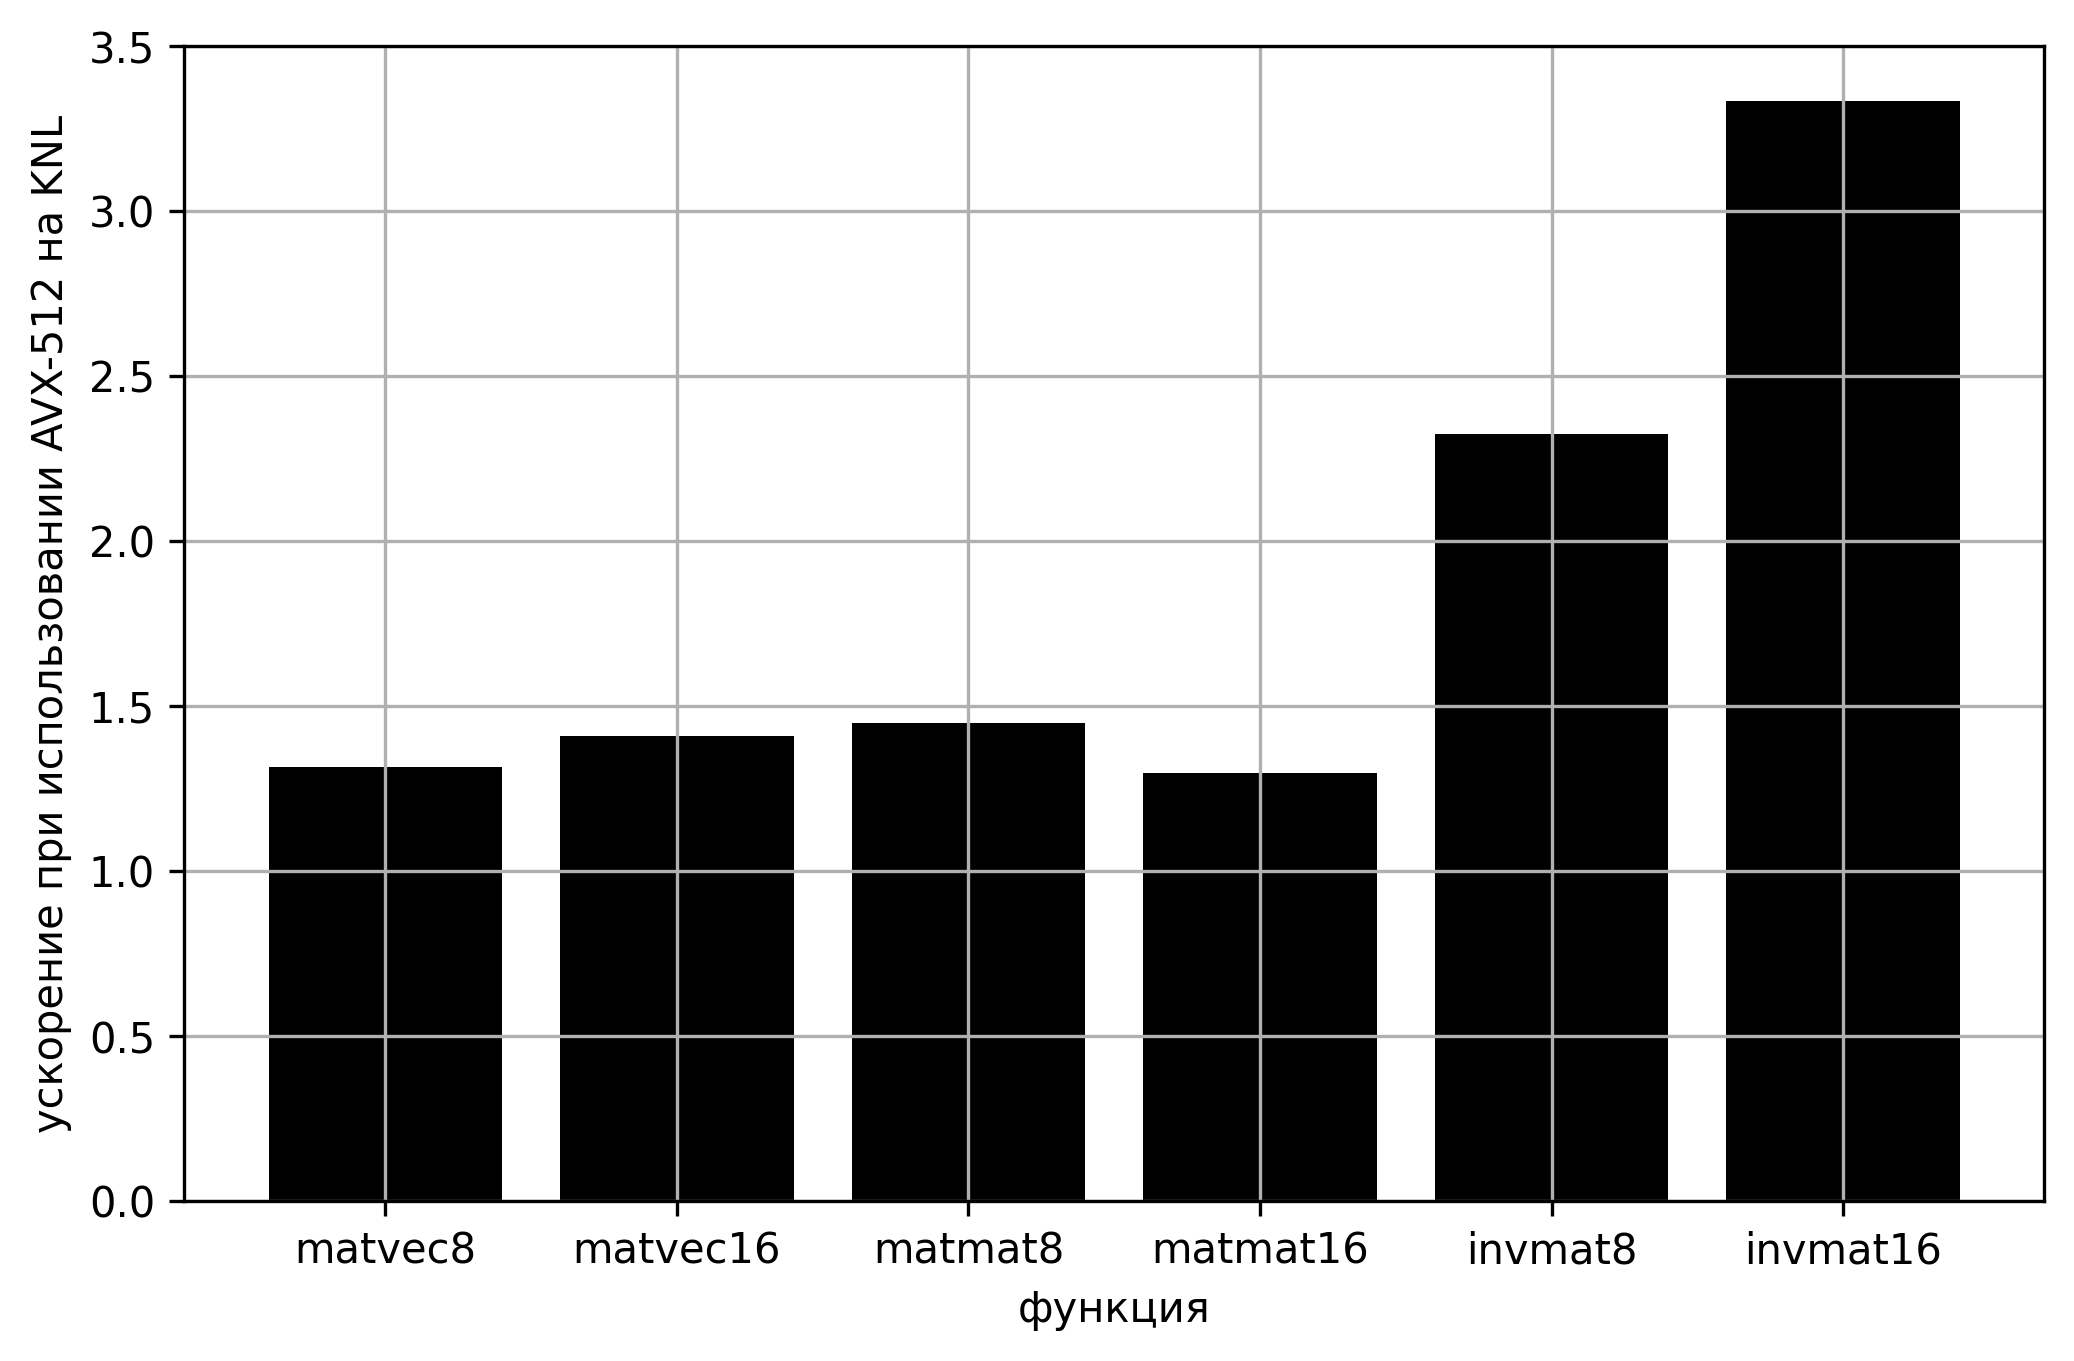
\includegraphics[width=0.6\textwidth]{./pics/text_4_small_matr/res.png}
\singlespacing
\captionstyle{center}\caption{Ускорение и эффективность векторизации операций над матрицами размера $8 \times 8$ и $16 \times 16$.}
\label{fig:text_4_small_matr_res}
\end{figure}

Наибольшее ускорение продемонстрировали функции нахождения обратной матрицы, так как алгоритм нахождения обратной матрицы естественным образом формулируется в терминах работы со строками объединенной матрицы, что находит свое отражение в 512-битных векторных операциях.
При этом функция \texttt{invmat16} ускорилась больше, чем \texttt{invmat8}, потому что, в отличие от \texttt{invmat8}, она не содержит накладных действий, связанных с копированием входной матрицы во временную матрицу, а затем чтением результата из временной матрицы.
Функции \texttt{matvec8/16} и \texttt{matmat8/16} демонстрируют умеренное ускорение.
Причиной тому служит наличие горизонтальных операций сложения, которые порождают длинный критический путь исполнения\label{term:critical_path2} внутри функции.
Объединение горизонтальных операций позволяет сгладить этот эффект, однако для дальнейшего ускорения требуется реализация объединенных функций, выполняющих одновременно сразу несколько операций или применяющих одну операцию к более широкому набору данных (например, функция перемножение двух пар матриц).
